\label{rzeczy_do_zrobienia_po_instalacji}
\subsubsection{Aktualizacja systemu}
\begin{wrapfigure}{R}{0.1\textwidth}
	\vspace{-10pt}
	
\includegraphics[width=\linewidth]{images/pierwsze_uruchomienie_aktualizacja1.png}
\end{wrapfigure}

Kliknij ikonę Dasha 
\includegraphics[scale=0.35]{images/ikony_dash.png} i wpisz \textcolor{ubuntu_orange}{Aktualizacje}. W trakcie wpisywania na ekranie wyników będą się pojawiały propozycje. Wybierz kolejno \menu{{Programy}>{Aktualizacje oprogramowania}}.
System sprawdzi, czy dostępne są aktualizacje dla twojego Ubuntu i wyświetli podsumowanie.

\begin{center}
	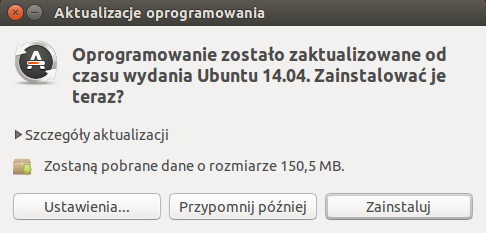
\includegraphics[width=\linewidth]{images/pierwsze_uruchomienie_aktualizacja2.png}
\end{center}

Kliknij przycisk \textcolor{ubuntu_orange}{Zainstaluj}, aby zainstalować aktualizacje. Zostaniesz poproszony o podanie hasła w celu uwierzytelnienia. Każda operacja mająca wpływ na cały system wymaga potwierdzenia. Zapobiega to przypadkowemu uszkodzeniu systemu.

\begin{center}
	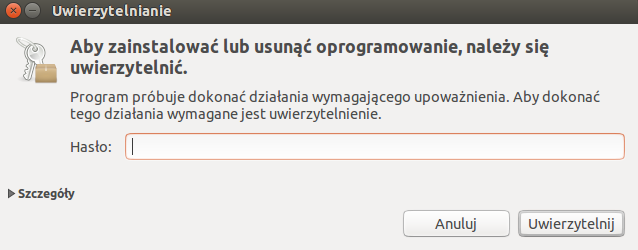
\includegraphics[width=\linewidth]{images/unity_uwierzytelnienie.png}
\end{center}

Wpisz swoje hasło i potwierdź klawiszem Enter lub kliknij przycisk \textcolor{ubuntu_orange}{Uwierzytelnij}. Teraz rozpocznie się proces pobierania i instalacji aktualizacji. To może potrwać od kilkunastu sekund do kilku minut, w zależności od tego, jak długo system nie był aktualizowany.

Kiedy aktualizacja się zakończy, możesz zostać poproszony o ponowne uruchomienie komputera. Restart jest potrzebny tylko wtedy, gdy aktualizowane było jądro systemu lub sterowniki. Inne aktualizacje nie wymagają restartu komputera, a jedynie zaktualizowanego programu.

Później system będzie automatycznie sprawdzał czy dostępne są aktualizacje i powiadomi cię o~tym.
\clearpage
\subsubsection{Instalacja spolszczenia}
\begin{wrapfigure}{R}{0.1\textwidth}
	\vspace{-10pt}
	
\includegraphics[width=\linewidth]{images/pierwsze_uruchomienie_lang1.png}
\end{wrapfigure}

Jeżeli w trakcie instalacji systemu nie wybrałeś języka polskiego lub nie miałeś połączenia z internetem, to tutaj dowiesz się, jak ściągnąć potrzebne paczki językowe i zainstalować odpowiednie oprogramowanie.
Kliknij ikonę Dasha 
\includegraphics[scale=0.35]{images/ikony_dash.png} i wpisz \textcolor{ubuntu_orange}{Języki}. System sprawdzi stan spolszczenia systemu i zaproponuje instalację dodatkowych paczek. Kliknij \textcolor{ubuntu_orange}{Zainstaluj}, a następnie potwierdź operację. Wpisz swoje hasło i potwierdź klawiszem Enter lub kliknij przycisk \textcolor{ubuntu_orange}{Uwierzytelnij}.

\begin{center}
	\vspace{-10pt}
	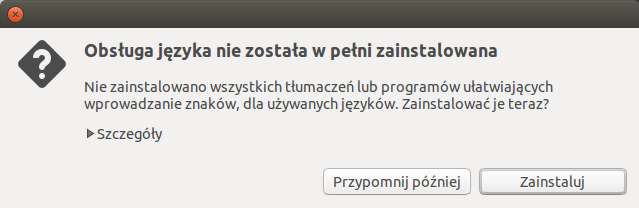
\includegraphics{images/pierwsze_uruchomienie_lang2.png}
\end{center}

Po instalacji niezbędnych paczek możesz jeszcze dla pewności kliknąć \textcolor{ubuntu_orange}{Zastosuj dla całego systemu}. W ten sposób będziesz pewny, że cały system zostanie spolszczony.
Jeśli zechcesz, aplikacja \textcolor{ubuntu_orange}{Języki} pozwoli ci później w łatwy sposób zainstalować i zmienić język systemu na każdy ze wspieranych przez społeczność Ubuntu.
\clearpage
\subsubsection{Instalacja dodatkowych sterowników}
\label{pierwsze_uruchomienie_aktualizacja_instalacja}
\begin{wrapfigure}{R}{0.1\textwidth}
	\vspace{-10pt}
	
\includegraphics[width=\linewidth]{images/pierwsze_uruchomienie_driver1.png}
\end{wrapfigure}

Prawdopodobnie nie wszystkie sterowniki zostały włączone podczas instalacji Ubuntu. Aby się upewnić, że sprzęt jest prawidłowo obsługiwany, kliknij ikonę Dasha 
\includegraphics[scale=0.35]{images/ikony_dash.png} i wpisz \textcolor{ubuntu_orange}{Sterowniki}. Z wyświetlonych wyników wybierz ,,Aktualizacje i sterowniki''. W otwartym oknie przejdź do zakładki ,,Dodatkowe sterowniki''. Poczekaj chwilę, aż system zbierze dane o twoim komputerze i porówna je z bazą danych sterowników. Następnie będziesz mógł wybrać, który sterownik z wyświetlonej listy powinien zostać użyty.
\begin{center}
	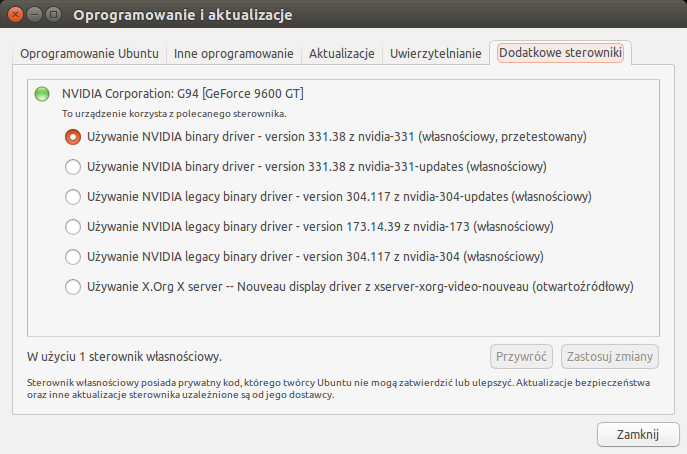
\includegraphics[width=\linewidth]{images/pierwsze_uruchomienie_driver2.png}
\end{center}

Zmiana sterownika wymaga potwierdzenia. Wpisz swoje hasło i potwierdź klawiszem Enter lub kliknij przycisk \textcolor{ubuntu_orange}{Uwierzytelnij}. Więcej o wyborze sterownika przeczytasz w rozdziale \ref{sterowniki},,Sterowniki''.

\subsubsection{Instalacja dodatków}
\label{ubuntu-restricted-extras}
\begin{wrapfigure}{R}{0.1\textwidth}
	\vspace{-10pt}
	
\includegraphics[width=\linewidth]{images/pierwsze_uruchomienie_dodatki1.png}
\end{wrapfigure}

Na koniec warto zainstalować kilka dodatkowych pakietów oprogramowania. Kliknij ikonę Dasha 
\includegraphics[scale=0.35]{images/ikony_dash.png} i wpisz \textcolor{ubuntu_orange}{Centrum Oprogramowania}. Z wiersza \textcolor{ubuntu_orange}{Programy} wybierz \textcolor{ubuntu_orange}{Centrum Oprogramowania Ubuntu}. W prawym górnym rogu nowo otwartego okna znajduje się pole wyszukiwania. Wpisz w nim \textcolor{ubuntu_orange}{Ograniczone dodatki Ubuntu} i wciśnij Enter. Poczekaj, aż odnaleziona zostanie ta paczka. Z listy wybierz \textcolor{ubuntu_orange}{Ubuntu restricted extras} i kliknij \textcolor{ubuntu_orange}{Zainstaluj}. Instalacja oprogramowania wymaga uwierzytelnienia. Wpisz swoje hasło i potwierdź klawiszem Enter lub kliknij przycisk \textcolor{ubuntu_orange}{Uwierzytelnij}.
\begin{center}
	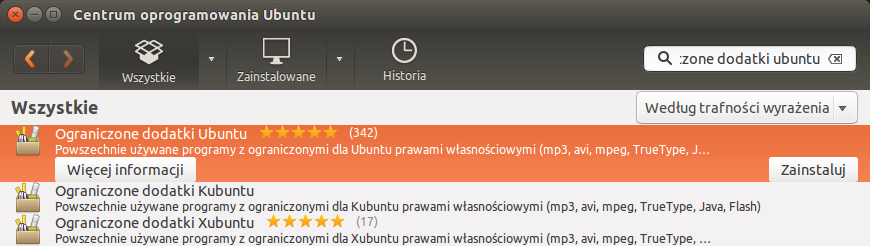
\includegraphics[width=\linewidth]{images/pierwsze_uruchomienie_dodatki2.png}
\end{center}

Paczka \textcolor{ubuntu_orange}{ubuntu-restricted-extras} zawiera:
\begin{itemize}
\item wszystkie możliwe kodeki audio/wideo;
\item odtwarzacz Flash;
\item fonty True Type (np. Times New Roman).
\end{itemize}
W podobny sposób wyszukaj i zainstaluj programy \textcolor{ubuntu_orange}{openjdk-7-jre} (Java, potrzebna do wielu popularnych programów), \textcolor{ubuntu_orange}{unzip} (obsługa archiwów zip), \textcolor{ubuntu_orange}{unace} (windowsowe archiwa ace) i \textcolor{ubuntu_orange}{p7zip-full} (obsługa archiwów w formacie 7z/lzma).
\clearpage
